%%%% Proceedings format for most of ACM conferences (with the exceptions listed below) and all ICPS volumes.
\documentclass[sigconf, final]{acmart}
%%%% As of March 2017, [siggraph] is no longer used. Please use sigconf (above) for SIGGRAPH conferences.

%%%% Proceedings format for SIGPLAN conferences 
% \documentclass[sigplan, anonymous, review]{acmart}

%%%% Proceedings format for SIGCHI conferences
% \documentclass[sigchi, review]{acmart}

%%%% To use the SIGCHI extended abstract template, please visit
% https://www.overleaf.com/read/zzzfqvkmrfzn


\usepackage{booktabs} % For formal tables
\usepackage{graphicx}

% Copyright
%\setcopyright{none}
%\setcopyright{acmcopyright}
%\setcopyright{acmlicensed}
\setcopyright{rightsretained}
%\setcopyright{usgov}
%\setcopyright{usgovmixed}
%\setcopyright{cagov}
%\setcopyright{cagovmixed}


% DOI
\acmDOI{10.475/123_4}

% ISBN
\acmISBN{123-4567-24-567/08/06}

%Conference
\acmConference[WOODSTOCK'97]{ACM Woodstock conference}{July 1997}{El
  Paso, Texas USA}
\acmYear{1997}
\copyrightyear{2016}


\acmArticle{4}
\acmPrice{15.00}

% These commands are optional
%\acmBooktitle{Transactions of the ACM Woodstock conference}
\editor{Jennifer B. Sartor}
\editor{Theo D'Hondt}
\editor{Wolfgang De Meuter}


\begin{document}
\title{A platform for massive data transformation and linking}
%\titlenote{Produces the permission block, and copyright information}
\subtitle{The EW-Shopp approach}
%\subtitlenote{The full version of the author's guide is available \texttt{acmart.pdf} document}


\author{Ben Trovato}
%\authornote{Dr.~Trovato insisted his name be first.}
\orcid{1234-5678-9012}
\affiliation{%
  \institution{Institute for Clarity in Documentation}
  \streetaddress{P.O. Box 1212}
  \city{Dublin}
  \state{Ohio}
  \postcode{43017-6221}
}
\email{trovato@corporation.com}

\author{Michele Ciavotta}
%\authornote{The secretary disavows any knowledge of this author's actions.}
\affiliation{%
  \institution{Institute for Clarity in Documentation}
  \streetaddress{P.O. Box 1212}
  \city{Dublin}
  \state{Ohio}
  \postcode{43017-6221}
}
\email{webmaster@marysville-ohio.com}

\author{Lars Th{\o}rv{\"a}ld}
%\authornote{This author is the one who did all the really hard work.}
\affiliation{%
  \institution{The Th{\o}rv{\"a}ld Group}
  \streetaddress{1 Th{\o}rv{\"a}ld Circle}
  \city{Hekla}
  \country{Iceland}}
\email{larst@affiliation.org}



% The default list of authors is too long for headers.
\renewcommand{\shortauthors}{B. Trovato et al.}


\begin{abstract}
This paper aims at presenting the subsystem of a comprehensive platform dedicated to the data transformation, linking and extension of massive data sets. The main requirements that have led the design and development of the platform are also detailed and discussed as well as the devised approach as direct consequence of the requirement elicitation and discussion phase. In particular,  both design time and run time aspects of the data transformation process are supported and this can be seen reflected in the architecture. 
Some initial tests have been carried out on data sets of a TB featuring promising performance. 
\end{abstract}

%
% The code below should be generated by the tool at
% http://dl.acm.org/ccs.cfm
% Please copy and paste the code instead of the example below.
%
\begin{CCSXML}
<ccs2012>
 <concept>
  <concept_id>10010520.10010553.10010562</concept_id>
  <concept_desc>Computer systems organization~Embedded systems</concept_desc>
  <concept_significance>500</concept_significance>
 </concept>
 <concept>
  <concept_id>10010520.10010575.10010755</concept_id>
  <concept_desc>Computer systems organization~Redundancy</concept_desc>
  <concept_significance>300</concept_significance>
 </concept>
 <concept>
  <concept_id>10010520.10010553.10010554</concept_id>
  <concept_desc>Computer systems organization~Robotics</concept_desc>
  <concept_significance>100</concept_significance>
 </concept>
 <concept>
  <concept_id>10003033.10003083.10003095</concept_id>
  <concept_desc>Networks~Network reliability</concept_desc>
  <concept_significance>100</concept_significance>
 </concept>
</ccs2012>
\end{CCSXML}

\ccsdesc[500]{Computer systems organization~Embedded systems}
\ccsdesc[300]{Computer systems organization~Redundancy}
\ccsdesc{Computer systems organization~Robotics}
\ccsdesc[100]{Networks~Network reliability}


\keywords{ACM proceedings, \LaTeX, text tagging}


\maketitle


\section{Introduction}

EW-Shopp aims to support e-commerce, retail and marketing industries in improving their efficiency and competitiveness through providing the ability to perform predictive and prescriptive analytics over integrated and enriched large datasets through the use of open and flexible solutions. 
This document is intended to be the first step towards the construction of the EW-Shopp ecosystem, a platform that seeks to significantly reduce integration time and to improve the quality of analytics by providing cutting-edge tools and access to data as a service, with particular reference to weather and event information.  


For some years now we have been witnessing the flourishing and reinforcement of Big Data methodologies in academia and especially in industry. 
This success can be partly explained by the promise of Big Data supporters to define and deliver more accurate and efficient data-driven decision-making processes.
This is not the only asset, but it is what we are most interested in highlighting within the EW-Shopp project. 
The term "Data Analytics" is too often used to define a generic data driven decision process and therefore covers heterogeneous activities such as cleaning, linking, enrichment/extension, application of analytic models up to business intelligence and visualization. 
In this document, we propose to design a platform from its components and their relationships. We present a reference architecture obtained from a rigorous process of requirements elicitation that took into account both literature and best practices as well as the needs expressed by involved stakeholders. 
A considerable amount of work has already been done within the consortium (presented in document D4.1 [1]) to outline the strategy for the implementation of business case pilots. In that particular document, not only the functional requirements associated with business cases (the implementation and reporting of which in marketed services is one of the core aspects of the project) have been collected and refined, but also the development guidelines based on lean methodology [2] have been defined. In particular, the build-measure-learn feedback loop is also presented. In a nutshell, the methodology envisions for each pilot a starting phase with Minimum Viable Product (MVP) meant to reduce the time-to-market. The MVP is going to be enriched as the project progresses and the vision matures. Pilots are therefore seen as playgrounds for experimenting approaches and technologies that eventually will be included in the final marketed services. 
Three stages of the development are foreseen:
\begin{itemize}
    \item First stage is building the integrated data platform from heterogeneous sources as the key inputs. 
    \item In the second stage the technical partners will need to present is analytical expertise to model these data to extract relevant analytical patterns, predictive strength and business sense.
    \item The last stage will be the development of marketed services focused on target segments on top of the integrated platform.
\end{itemize}

At the time this document is written, we are at the beginning of the first phase and it is the right time to design a unified, complete and well-founded reference architecture. The declared objective is to provide a point of reference that will remain as steady as possible for the entire duration of the project and that can thus lead its evolution on the basis of a solid and agreed basis. To do this, as we will see, we started from the functional requirements collected in D4.1 trying to read in them the answers to the architectural questions that we asked ourselves.  It was immediately evident, however, that these requirements were not sufficient to define a modern, efficient, responsive and scalable platform. As a consortium, we have therefore decided to undertake an in-depth study of the problems that we want to tackle. The results of such teamwork are detailed in this document.  

With the work the consortium has done on component design, the processes and outcomes of which are described in this document, we aim to achieve the following two objectives:
1.	Define a reference architecture. This deliverable provides a reference architecture that aims at being general and flexible enough to be successful applied in the pilots. The architecture describes the core components and their relationships in terms of data flow. Moreover, it aims at setting a common language among the partners. To make this possible, we have referred to the pilot descriptions, the partners’ experience, and the best practices of the field of Big Data. Furthermore, the effort required to define precisely the pilots, especially in terms of processes, data flow and workflow, has spawned awareness in the consortium members about the complexity of the problem and the need of a common reference. Finally, it is important to note that defining a reference architecture does not conflict with the lean methodology as we describe the components according to their general functionality, without imposing specific solutions.
2.	Propose an initial implementation of the platform. This deliverable also provides an early stage implementation of the reference architecture, whose components can be divided into two groups; the first one contains tools upon which there is a general agreement among the partners, the second one features components that are either left unspecified or are concrete tool to be considered as an initial choice (subject to be further refinement). Such an approach is necessary for two reasons. First of all, following the lean methodology the pilots need freedom to experiment in order to make the platform evolve. Secondly, part of the ecosystem must be adaptable to the needs of individual pilots, which might require the use of specific technologies.  


This work is structured as follows. In Chapter 2 we present the reference architectures for Big Data as well as the main solutions for data wrangling, data analytics, business intelligence and reporting. The requirements that have guided the definition of our reference architecture are presented and discussed in Chapter 3. The EW-Shopp reference platform is detailed in Chapter 4, where both the reference data flow and control flow are also presented. Once the reference architecture has been defined, we have decided to present a possible implementation (in embryonic form) of the EW-Shopp platform in Chapter 5. Finally, Chapter 6 concludes the document. 









\section{Platform Design}\label{sec:approach}

In this section, we outline the guiding principles behind the current platform architecture. 
In order to precisely identify the main application scenarios and objectives, a thorough requirement gathering phase has been carried out taking into account the first principles underpinning Big Data solutions and the expectations of the business partners involved in the project. The main requirements drove the core design of the platform. As the platform deals with issues of data processing, integration, enrichment, and extension, it needed to support data flow definition and execution. 
Furthermore, EW-Shopp business cases provided input data sets in tabular format from heterogeneous domains, and of different volumes, including Big Data. In many cases, the data provided by organizations was a core asset and thus, also data confidentiality needed to be retained. 
Due to the varying security requirements of organizations, the system had to be designed to flexibly support different security setups. The data flows themselves had to be defined on a high level and composed of independent steps, which also include data integration and enrichment at scale. Finally, deployment of the flows had to be flexible in terms of both hardware and software, so that they can be deployed in different infrastructures that fit organizational needs best.
The main specific platforms for data wrangling available on the market have been also evaluated, and in particular, OpenRefine\footnote{\url{http://openrefine.org/}}, Trifacta Wrangler\footnote{\url{https://www.trifacta.com/products/wrangler/}} and Karma\footnote{\url{http://usc-isi-i2.github.io/karma/}}. 

At the end of this process, the need for an \textit{open source} platform, capable of managing data in \textit{tabular format} and of generating \textit{linked data}, became clear. 
In addition, two possible use cases have emerged. In the first case, small amounts of data have to be manipulated, the platform has to be lean and \textit{easy to install on a commodity machine} similarly to tools like OpenRefine. In the second scenario, a genuinely big data must be managed, this means that a domain expert user must be able to describe the transformation through a user-friendly and interactive interface and to execute it in an automated way as a \textit{batch} process (as in Karma and Trifacta Wrangler). 
Common to both scenarios is the need to supply linking and enrichment services to manage \textit{geocoding}, \textit{schema linking}, \textit{entity linking} and extension with \textit{weather} and \textit{events} data. 

In an attempt to give a syncretic response to the needs outlined in the requirements, we have based platform design on two fundamental driving principles:  \textit{Separation of Concerns} and \textit{Dimension Reduction}.  
In particular, by applying separation of concerns, we have conceived the platform as composed of three tiers (Figure~\ref{fig:architecture}):

\begin{description}
    \item[Core Data Services] (in light blue): These components provide access to corporate on-boarding or third party data. These data sets are used in both data linking and extension processes. Figure~\ref{fig:architecture} shows services to access the project's core data, i.e., weather (W), events (E) and Products (P). Other enrichment sources may include services as Wikifier\footnote{\url{http://wikifier.org/}}, and freely accessible knowledge bases such as DBpedia\footnote{\url{https://wiki.dbpedia.org/}}.
    \item[Platform Services] (in green): data preparation, analytics and visualization services (the last two are not addressed in this paper). These services offer simple and intuitive user interfaces for creating (and executing if the working table is small enough) data wrangling, linking and extension pipelines.
    \item[Corporate Services] (in red): These services implement platform components needed for data governance, i.e., ingestion, storage, processing, data flow and security management of massive data sets. This tier is used to perform data wrangling operations at scale. 
\end{description}


The rationale of the Dimension Reduction~\cite{rojas2017sampling, ur2016big} approach in Big Data is also rather simple in its general lines; it consists in reducing the size of the data set by identifying a possible compact representation (i.e., a subset of data plus a profile). In this way, the data transformation operations can be designed and tested on a set that can be several orders of magnitude smaller than the original. This should ensure greater responsiveness and efficiency for the applications involved without negatively affecting accuracy. For this reason, we have introduced into the platform a specialized component, whose task is to properly generate this data subset. 
We remark that the presented design choices do not reduce the applicability and generality of the presented architecture as, where it is possible (e.g., in cases where the data to be transformed is manageable), the corporate subsystem can be excluded. In this mode, the user can work directly against the original data set.


 
\begin{figure}[t]
\centering
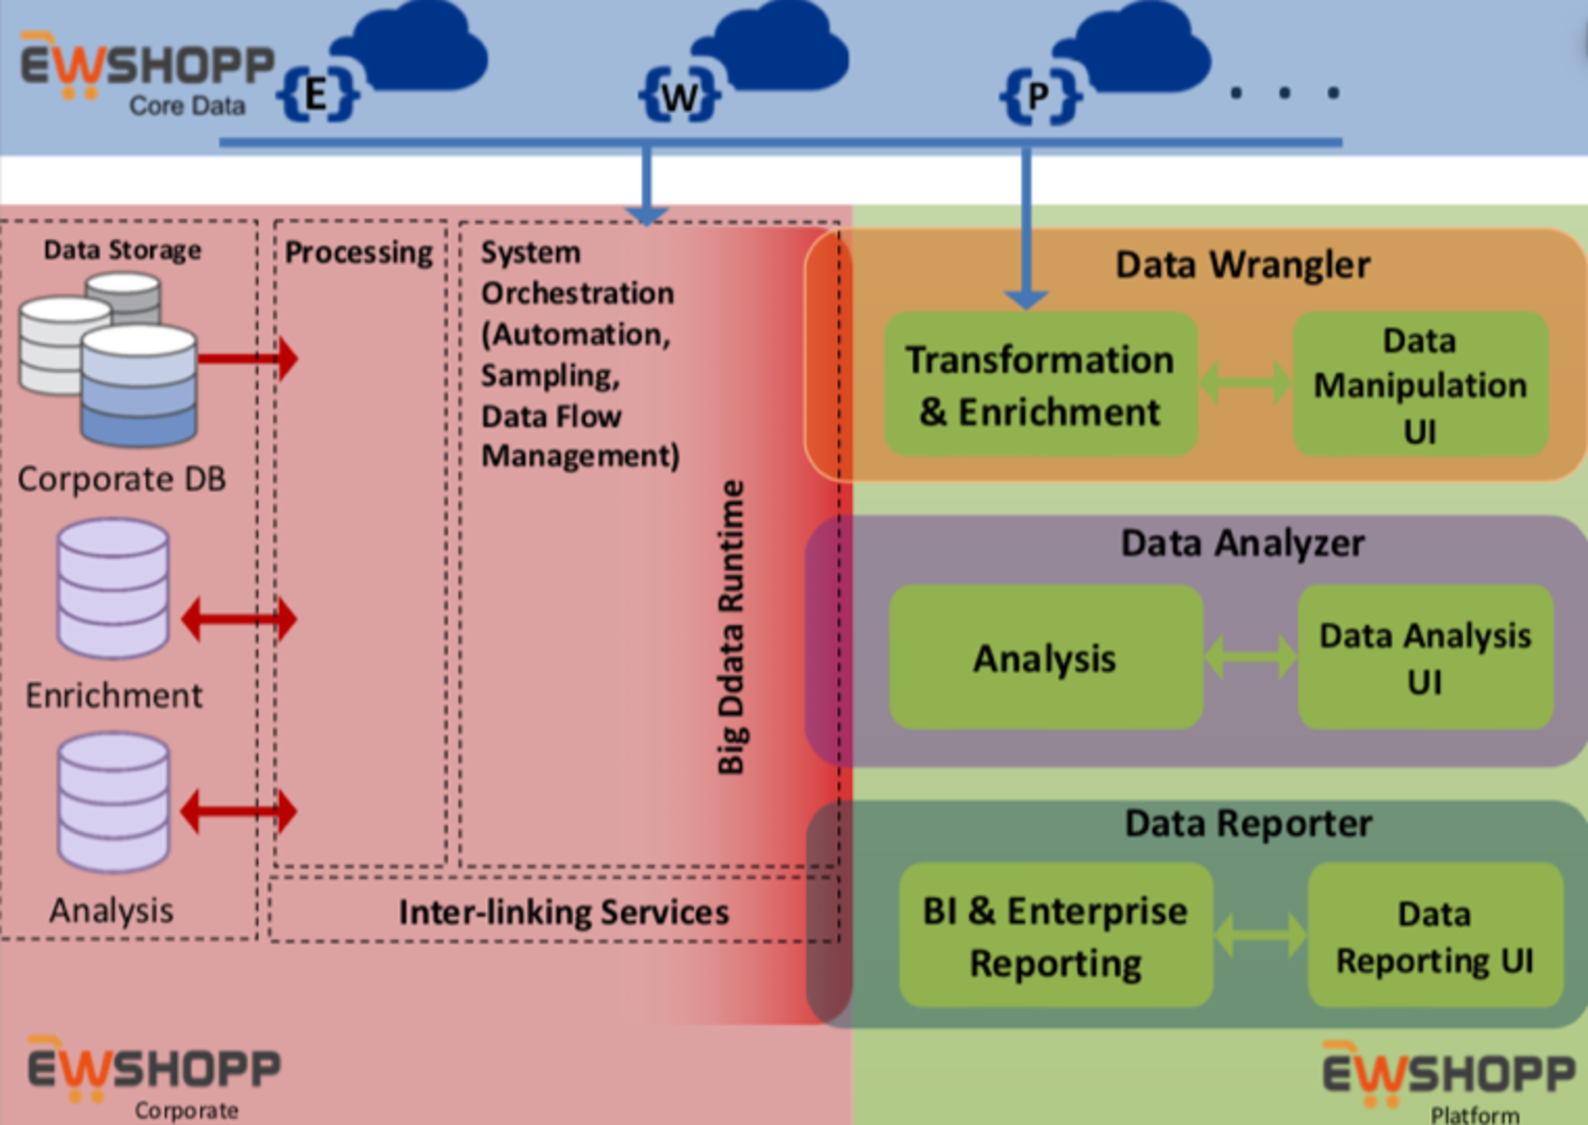
\includegraphics[width=\columnwidth]{figs/Architecture.pdf}
%\vspace{-.3cm}
\caption{General architecture}
\label{fig:architecture} 
\end{figure}  




%- open source
%- linking data
%- data onboarding https://www.trifacta.com/blog/data-onboarding-broken-matters/
%- sampling
%- backend batch execution
%- wrangling separato per essere usato cosi com'è per evitare di installare e gestire la piattaforma retrostante.
%- Servizi di interlinking e estensione
%- Gestione dei dati core del progetto. 




%The EW-Shopp system aims to support e-commerce, retail and marketing industries in improving their efficiency and competitiveness through providing the ability to perform predictive and prescriptive analytics over integrated and enriched large data sets using open and flexible solutions. 
%In addition, these tools must provide a responsive graphical user interface to guide the user in designing data transformations. 
 
\section{Data Wrangling at Scale}\label{sec:architecture}
As mentioned above, in the designed architecture a logical separation between  platform and corporate services has been imposed. This structure is conceived to make the architecture flexible and adaptable to different deployment scenarios. 
In what follows, the main components and interaction of the platform are presented. 

Figure~\ref{fig:wrangler} shows a component diagram of our wrangling solution with component interactions and information flows. 
The image presents the most general case, where the data set to be transformed is genuine Big Data and, for this reason it is managed by the corporate services. 
In this scenario, components from all logical areas are involved; we have on the left a corporate component called \textit{Sampler} , the \textit{Summarizer} and the \textit{Engine} that are the components that are entrusted of creating the (reduced) working data set to be used to define the transformations, of providing a set of suggestions for the table annotation process based on summaries of existing knowledge bases or previous annotations, and finally, of interacting with the \textit{Big Data Runtime} to carry out on a large scale the transformations defined by the user, respectively. 
\begin{figure}[t]
    \centering
    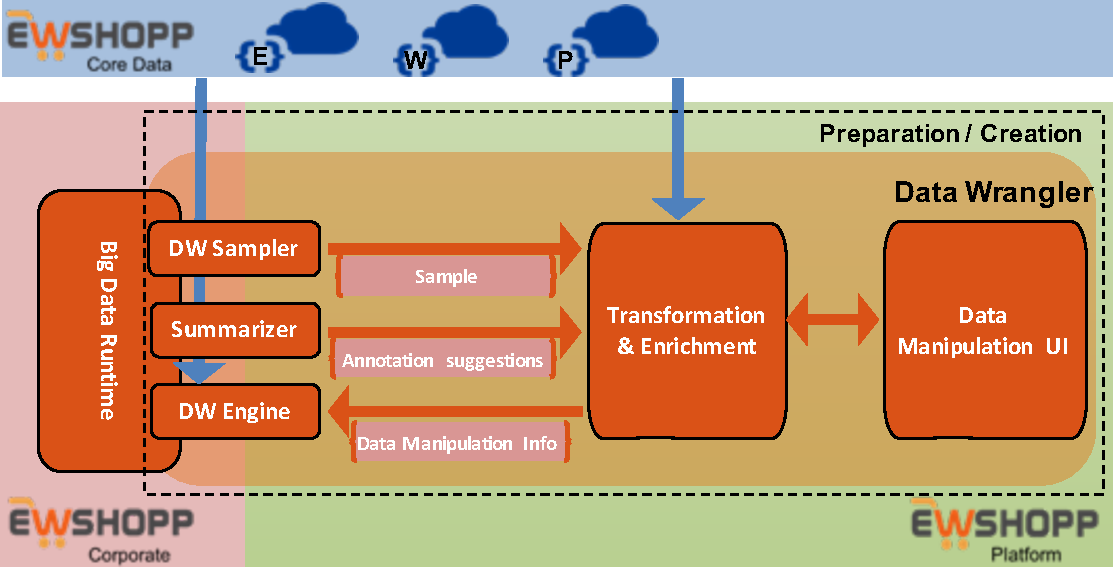
\includegraphics[width=\columnwidth]{figs/Wrangler.pdf}
    \caption{Data Wrangler's components and interactions}
    \label{fig:wrangler} 
\end{figure}  
The definition of the transformation pipeline, instead, is carried out using the platform services, depicted in the right side of the Figure. In particular, the user is supported in this task by a graphical manipulation interface, which in turn interacts with a \textit{Transformation and Enrichment} back-end service. This service has the twofold duty of executing the pipeline on the reduced data set, thus allowing the platform to be used as a standalone solution, and of interacting with the corporate services. In both cases, core data services support linking and extension capabilities. 

The architecture and components interactions within the Big Data Runtime are depicted in Figure~\ref{fig:big_data_runtime}. The \textit{System Orchestration} sub-component is used to define the high-level data flows that will be executed by \textit{Processing} tool. Such Data flows include the data wrangling pipelines but they may also incorporate pre- and post-processing steps, e.g, automatic obtaining of data, re-formatting, import to data warehouse (enrichment database). The end result is a data flow that can be deployed as a Function as a Service (FaaS) computing service over a managed cluster of resources, which allows for easy integration with business processes and heterogeneous infrastructures (see Section~\ref{sec:bdr}).

For sake of clarity a high-level workflow is reported:
\begin{enumerate}
    \item A reduced data set (possibly complemented by profiling information) is created and passed to the \textit{Transformation and Enrichment} component.
    \item The user operates the \textit{Data Manipulation UI}, which also interacts with the Core Data services and \textit{Summarizer} to perform schema and entity linking, to extend the data with weather and events information.
    \item The application generates a self-contained machine-runnable pipeline of the user's operations which is eventually executed on the original data set by the \textit{Big Data Runtime}. 
\end{enumerate}

\begin{figure}[t]
    \centering
    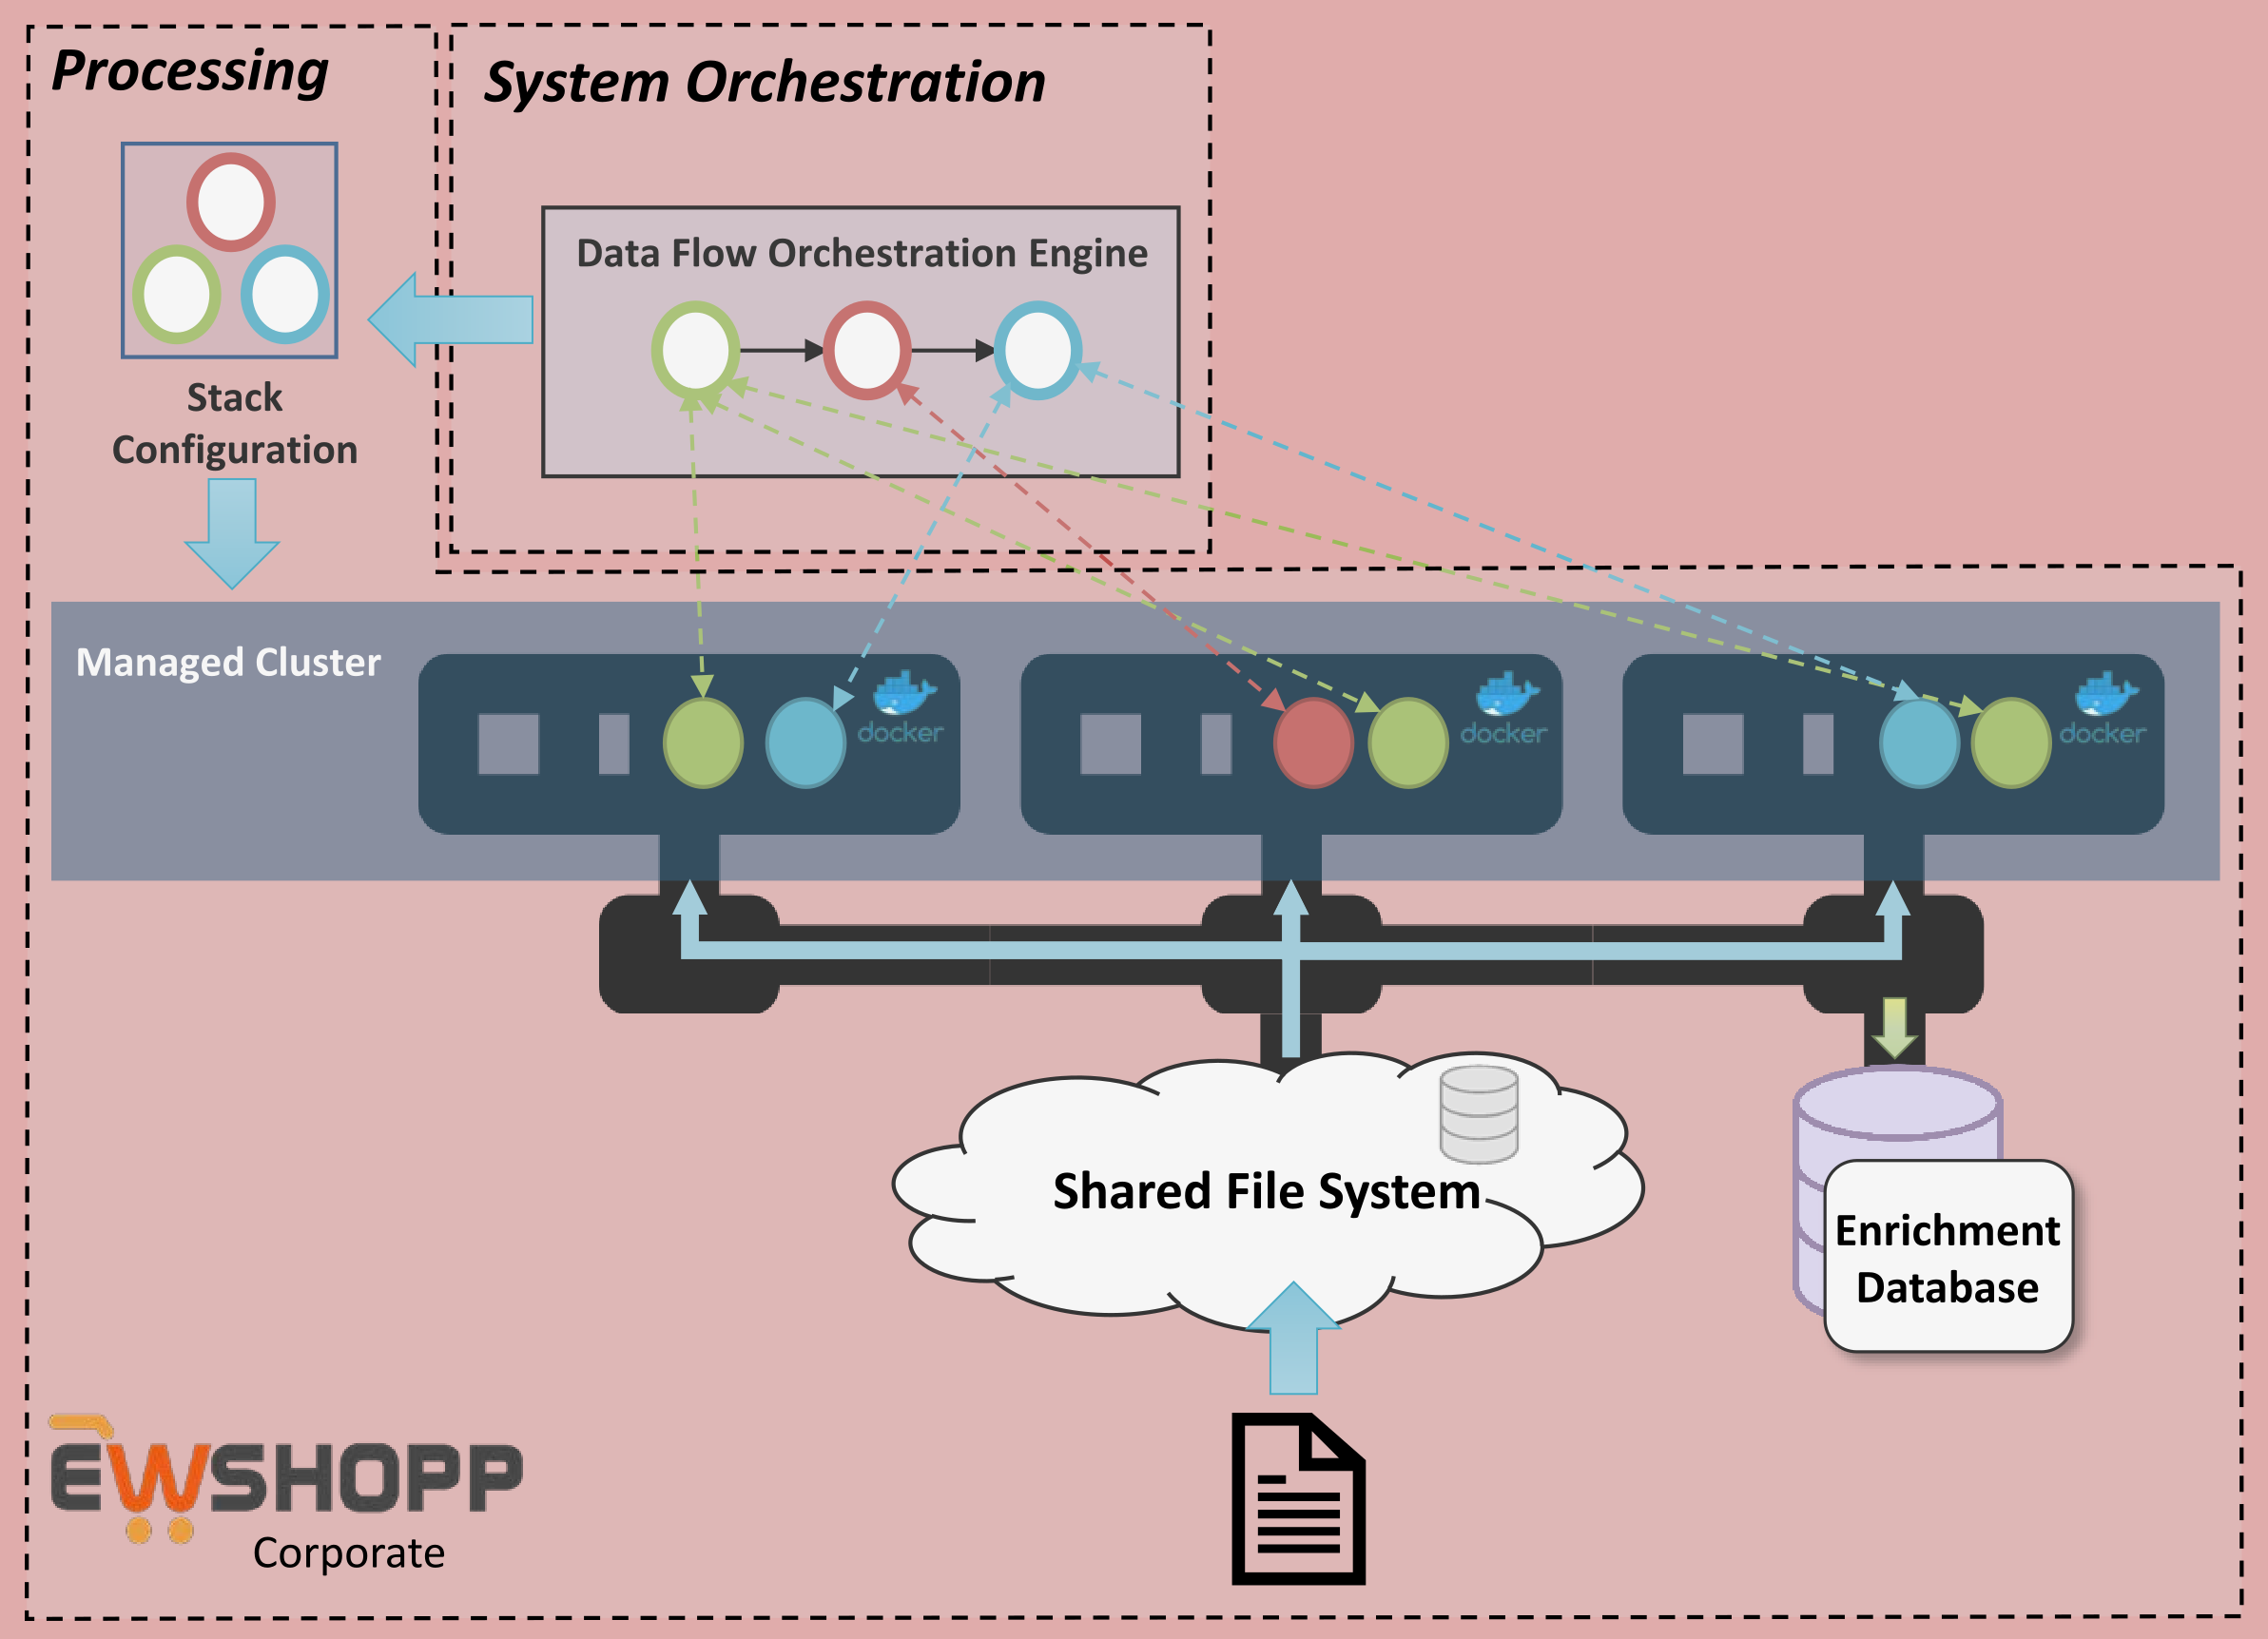
\includegraphics[ width=0.9\columnwidth]{figs/SACBD2018-Big-data-processing-engine.png}
    \caption{Big Data Runtime components interaction}
    \label{fig:big_data_runtime} 
\end{figure}  

The next two subsections detail the components and interactions of the proposed solution, highlighting which components are involved at design time and which at run time. 


\subsection{Platform services}

The Data Wrangler is a composite component built upon the DataGraft platform~\cite{roman2016datagraft}, extended with semantic enrichment and Big Data processing capabilities. DataGraft provides tools for cleaning and transformation of tabular data into RDF and graph generation mappings.
%featuring a composite architecture that follows the service-oriented architecture mandates. 
DataGraft comes with an interactive web application, named Grafterizer~\cite{sukhobok2016tabular}, which serves as user interface helping platform users to transform data from a tabular format into a graph format. The transformation supports both cleaning and graph mapping steps. Transformation steps on rows (add, drop, filter, duplicate detection etc.), columns (add, drop, rename, merge etc.) and entire data set (sort, aggregate etc.) are provided together with visualization of the result after each step. The mapping to ontologies or vocabularies is performed on the cleaned-up data. 
%Moreover, the DataGraft is responsible for user-facing miscellaneous tasks such as user management, managing user assets (i.e., Enrichment Database endpoints, queries, transformation models) and enabling easy access to data.  

As mentioned, the EW-Shopp platform aims to support scalable data enrichment. Therefore, DataGraft and the transformation tool, Grafterizer, incorporate two sub-components called ASIA and ABSTAT. The components provide functionalities for the semantic enrichment of data tables and profiling of knowledge graphs, respectively. ASIA is meant to aid users in integrating business data and can be used to map the data schema to shared vocabularies/ontologies, or link data values to shared systems of identifiers, which enables the extraction of additional data from third-party sources and their fusion into the original tabular data. Schema-level and instance-level links are created by ASIA as annotations for the table. ABSTAT~\cite{palmonari2015abstat} is a tool to profile knowledge graphs represented in RDF based on linked data summarization mechanisms. The profiles extracted by ABSTAT describe the content of knowledge graphs, using abstraction (schema-level patterns) and statistics. Such profiles are exploited by ASIA to provide the user with suggestions in schema linking activity. 


%Nikolay: too much low-level detail 
%Users can create schema-level annotations through the ASIA interface, by validating ASIA suggestions about classes and properties to be used. If a user specifies a different class (or property), ASIA suggests classes (or properties) that syntactically match the user input implementing the autocomplete functionality. Otherwise, the instance-level annotations are expected to be created by ASIA semi-automatically.

%Nikolay: too much low-level detail 
%As a matter of fact, summaries record rich statistics about the usage of vocabularies/ontologies in data sets. Thus, they can provide types and properties that match a string, for example, the header of a column in a table to be published. In addition, statistics provide valuable information to algorithms aimed at suggesting the best properties and types to use when transforming a tabular data into RDF.  
\subsection{Corporate Services}\label{sec:bdr}

%We have introduced the platform components in the previous section, in this section we focus on the services of the corporate section. In the most general case, these components are physically distant from the platform components and interact with them via APIs. 
%In the early stages of pilot development, we do not rule out the possibility that the interaction between the components of the two logic areas can be carried out manually by means of one or more human users.  

%The Big Data Runtime (BDR) component's role in our solution is to perform batch data cleaning, integration, enrichment and data transformation at scale. 
%The objective of the pipeline is to eventually expose the data in a central database for performing analytics.

The Corporate services of the EW-Shopp solution are mainly responsible for the orchestration and execution of wrangling operations at scale. 
In particular, based on the user-defined data wrangling pipeline (cleaning, transformation, graph mapping, enrichment, and extension) declared on the sampled data, a so-called transformation model is created and transmitted to the corporate services in order to be applied to the full data set. Once there, the model is compiled into a self-contained executable Java archive (JAR) and executed as the main step of a larger process that is referred to as Data Flow.  
Data Flows are  extension of the data wrangling pipeline with pre- and post-processing actions. 
To serve as an example, a data flow coming from a business case of EW-Shopp is described below:
\begin{enumerate}
    \item Decompress data - large data set is delivered as a set of archives contain CSV files, which are stored in a shared file system of our private cloud.
    \item Split data in chunks for faster processing and horizontal scalability of inputs.
    \item Execute the data wrangling pipeline - Clean up, re-format, transform, map to ontology, and enrich the split data. 
    \item Import the resulting data set into the Enrichment database
\end{enumerate}



The System Orchestration component provides a high-level interface to handle and monitor a data flows, whereas the Processing component is in charge of carrying them out. From the technological point of view, data flows are compiled into a chain of Docker\footnote{https://www.docker.com/} containers that are in turn deployed and run through a Container Orchestration system (e.g., Kubernetes\footnote{\url{https://kubernetes.io/}}, Rancher\footnote{\url{https://rancher.com/}}) on a cluster of machines connected via an Ethernet fabric and mounting a shared filesystem (e.g., GlusterFS\footnote{\url{https://www.gluster.org/}}).
The implementation of a container-based solution has several benefits; for instance, it allows to decouple the data flow deployment from the particular stakeholder's hardware infrastructure also working in heterogeneous distributed environments. Furthermore, it guarantees flexible deployments, better resource utilization, and seamless horizontal scalability.  

 
%Each machine runs the Docker engine, so that Docker containers can be deployed. The particular virtual hardware allocated to each of the Docker container that implement the processing pipeline depends on the load and is configurable. The deployment of Docker containers is controlled at run time by the container orchestration system. 
Finally, for the sake of completeness, the following non secondary aspects of the execution of a data flow are presented>
\begin{description}
    \item[Deployment of the flow configuration] - the flow configuration contains the context information to be fed to each step that compose the data flow, as well as any additional hardware constraints for each step. These parameters are passed to the containers in the chain they are intended for. Notice that an extensible library implements the most common (parametrized) actions to be used in the definition of a data flow. Moreover, each action implements a common interface to guarantee both composability and observability. 
    
    %in order to handle the scale of data, the Big Data Runtime component has to be able to distribute the individual workflow steps over a cluster of virtual machines (VMs) or containers. The cluster can be deployed on the premise of the EW-Shopp platform user to maintain the confidentiality of their data. The cluster also needs to provide access to the input data to all members of the cluster, for example by deploying data are on a reachable network location or on a mounted shared file system.
    \item[Execution of the data flow] - The Processing component establishes a suitable deployment in terms of machines and resources to be used and starts the appropriate number of containers for each step of the flow.  Each of the steps consists in a set of containers that work independently and in parallel, and can be scaled up or down on demand if required. The communication between two consecutive steps of the chain, that is the handover of the partial results, occur through writing and reading from file system in a specific way, defined in the context information.
%a specific way: each container is given an input, work and output folder and the cluster configuration reflects those settings. %Race conditions between individual containers that implement the steps are solved using low-level file operations.
    \item[Data Storage] - The results of the data flow can be stored on disk or (more typically) imported to an Enrichment Database. The database serves as a single source of truth to be used, for example, to slice and dice the data to obtain a subset needed for analytics or machine learning jobs. 
    %The Big Data Runtime deploys the output of the data workflow in a central data storage solution, which is accessible through the network, or deployed on the same cluster. 
\end{description} 
%The tools and services for providing analytics and reporting functions consume the data produced by the data workflow executed by the Big Data Runtime (BDR) through the central database. 
\section{Early evaluation}

- jot data
- some information about timing


\section{Conclusions}\label{sec:conclusions}
%The EW-Shopp ecosystem aims to support e-commerce, Retail and Marketing industries in improving their efficiency and competitiveness through providing the ability to perform predictive and prescriptive analytics over integrated and enriched large data sets using open and flexible solutions. 
In this paper, we have tried to pursue several objectives at once. Mainly, we have outlined a architecture specifically designed to transform, link and extend massive data sets supporting both design time and run time phases. 
This architecture is based on the principle of the data set Dimension Reduction that is an appropriate reduction the size of the data set, to make possible the agile definition a data enrichment process and the full-scale exectution of the resulting pipeline. 
Finally, we have tried to propose an initial implementation of the architecture by identifying one or more tools for each component of the reference architecture. In particular, at this stage we have embraced the lean development approach. Nevertheless, we believe that the reference architecture and its implementation will be able to guide the development process that will take place in the coming months.


\begin{acks}
  The work is
  supported by the \grantsponsor{GS501100001809}{National Natural
    Science Foundation of
    China}{http://dx.doi.org/10.13039/501100001809} under Grant
  No.:~\grantnum{GS501100001809}{61273304}
  and~\grantnum[http://www.nnsf.cn/youngscientists]{GS501100001809}{Young
    Scientists' Support Program}.

\end{acks}


\bibliographystyle{ACM-Reference-Format}
\bibliography{references}

\end{document}
